\documentclass[10pt]{article}
\usepackage{icmlko}

\icmlmeta{IP 파운데이션 월드모델}{190}{평평한 곡면에서 최댓값을 고르면 잡음을 고른다}{노트 189의 처방을 챔피언에 댔더니 거꾸로 갔다. 왜인지 갈랐고, 고를지 말지를 미리 정하는 지표 하나가 나왔다}

\begin{document}

\twocolumn[
\icmlheader

\begin{abstract}
노트 189가 능형 셋의 알파를 안쪽 시간 분할로 골라 $+$0.011$\sim$0.013 을
얻고 ``챔피언은 아직 안 조정했다''를 남겼다. 댔다. \textbf{거꾸로 간다} ---
격자 쉰넷을 훑어 안쪽이 고른 설정이 유보에서 $+$0.4490 을 \textbf{$+$0.4386}
으로 내린다($t{=}-2.44$). 표준 처방도 다 실패한다 --- 1-SE 풍(최댓값 근처에서
제일 단순한 것) $+$0.4196, 안쪽 상위 다섯 순위 평균 $+$0.4421, 열여덟 평균
$+$0.4419. \textbf{넷 다 손 안 댄 기본값보다 못하다.} 왜인지 갈랐다.
\textbf{안쪽 곡면이 평평하다} --- 격자 쉰넷의 상위 열이 \textbf{0.0026} 안에
몰려 있고, 안쪽 최고와 중앙의 차가 $+$0.0047 인데 유보에서 벌어진 차는
$-$0.0104 로 \textbf{두 배 넘게 크고 방향이 반대}다. 결정적으로
\textbf{현행 기본값은 안쪽에서 32/54 위인데 유보에서는 1위}다. 능형은
반대였다 --- 격자 일곱에서 안쪽이 뚜렷한 봉우리를 그리고(최고 0.5116 ·
중앙 0.4838) 그 봉우리가 유보로 그대로 옮겨 갔다. 그래서 지표 하나를
적는다: \textbf{봉우리 지수 $=$ (안쪽 최고 $-$ 안쪽 중앙) $\div$ (안쪽 최고
$-$ 안쪽 최저)}. 능형 셋이 \textbf{0.81 · 0.84 · 0.81} 이고 배깅 트리가
\textbf{0.129} 다. 네 점으로 스피어만 $+$0.80 이다. 문턱 0.5 로
\texttt{lab/tune.py} 에 넣었다 --- 평평하면 고르지 않고 기본값을 지킨다.
확인했다: F18 은 지수 0.138 로 막히고 능형 셋의 이득은 그대로다. 마지막으로
\textbf{열 번째 아티팩트}. 처음 잰 격자 스물일곱이 \emph{전부 정확히 같은}
안쪽 점수 0.5345 를 냈다 --- F18 의 깊이 · 반복 · 학습률이
\texttt{self.kw} 안에 \texttt{max\_depth} 따위로 들어 있어
\texttt{setattr(o, 'depth', 6)} 이 아무 데도 안 닿았다. \textbf{노트 187의
규약이 두 사이클 연속으로 잡았다.}
\end{abstract}
]

\begin{figure*}[t]
\centering
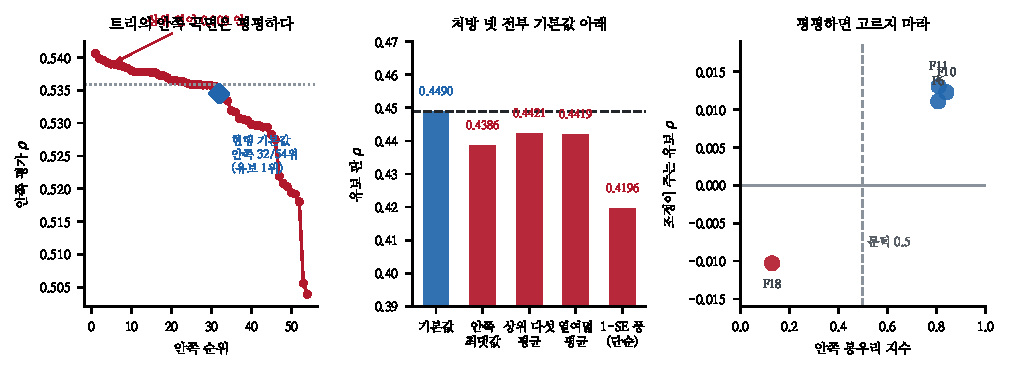
\includegraphics[width=\textwidth]{figs/flat.pdf}
\caption{왼쪽 --- 트리의 안쪽 곡면은 평평하다. 가운데 --- 처방 넷 전부
기본값 아래. 오른쪽 --- 평평하면 고르지 마라.}
\end{figure*}

\section{챔피언에서는 거꾸로 간다}

\begin{table}[t]
\centering\tsize
\caption{F18 배깅. 안쪽 격자 쉰넷(깊이 $\times$ 반복 $\times$ 학습률 $\times$ $l_2$).}
\begin{tabular}{lrl}
\toprule
& 유보 판 $\rho$ & \\
\midrule
\textbf{손 안 댄 기본값} & \textbf{.4490} & \\
안쪽 최댓값 & .4386 & $t{=}-2.44$ \\
안쪽 상위 다섯 평균 & .4421 & \\
격자 열여덟 평균 & .4419 & \\
1-SE 풍(제일 단순) & .4196 & \\
\bottomrule
\end{tabular}
\end{table}

\claimx{\textbf{처방 넷이 다 진다.} 최댓값도, 평균도, 단순한 쪽도 기본값을
못 넘는다.}{노트 189 에서 같은 절차가 능형 셋을 다 올렸다($t{=}4.5$ ·
$4.1$ · $1.8$). \textbf{절차가 아니라 대상이 문제다.}}

\section{안쪽 곡면이 평평하다}

\begin{table}[t]
\centering\tsize
\caption{안쪽 격자의 모양.}
\begin{tabular}{lrr}
\toprule
& F6 능형 & F18 트리 \\
\midrule
격자 크기 & 7 & 54 \\
안쪽 최고 & .5116 & .5406 \\
안쪽 중앙 & .4838 & .5359 \\
안쪽 최저 & .4772 & .5039 \\
\midrule
\textbf{최고 $-$ 중앙} & \textbf{$+$.0278} & \textbf{$+$.0047} \\
상위 열의 폭 & --- & \textbf{.0026} \\
\midrule
현행 기본값의 안쪽 순위 & --- & \textbf{32/54} \\
현행 기본값의 유보 순위 & --- & \textbf{1위} \\
\bottomrule
\end{tabular}
\end{table}

\claimx{\textbf{현행 기본값은 안쪽에서 32위인데 유보에서 1위다.} 그리고
안쪽 최고와 중앙의 차($+$0.0047)보다 유보에서 벌어진 차($-$0.0104)가 두 배
넘게 크고 방향이 반대다.}{\textbf{안쪽 신호가 안쪽 잡음보다 작다.} 그런
곡면에서 쉰넷 중 최댓값을 고르는 것은 잡음을 고르는 것이다 --- 격자가 클수록
심해진다.}

\claimx{왜 트리만 평평한가에 대한 읽기 하나 --- 안쪽 학습은 학습 구간의
앞 70\%라 행이 크게 줄고 도메인 셋(팝업 · 도서 · 아이돌)이 표본 부족으로
빠진다. \textbf{능형의 알파는 그 축소에 둔감하고 트리의 용량은
민감하다.}}{자료로는 못 가른다 --- 도메인을 유지한 채 행만 줄이는 실험이
필요한데 안 했다.}

\section{봉우리 지수}

\begin{table}[t]
\centering\tsize
\caption{(안쪽 최고 $-$ 중앙) $\div$ (안쪽 최고 $-$ 최저).}
\begin{tabular}{lrrl}
\toprule
& 지수 & 유보 차 & \\
\midrule
F10 도메인별 & \textbf{.841} & $+$.0123 & $t{=}1.80$ \\
F11 합집합 & \textbf{.810} & $+$.0131 & $t{=}4.06$ \\
F6 능형 & \textbf{.808} & $+$.0111 & $t{=}4.51$ \\
\midrule
\textbf{F18 배깅} & \textbf{.129} & \textbf{$-$.0103} & $t{=}-2.44$ \\
\bottomrule
\end{tabular}
\end{table}

\claimx{\textbf{0.81 대 0.13 으로 깨끗이 갈린다.} 스피어만 $+$0.80 인데
네 점이므로 세게 읽지 않는다 --- \textbf{읽을 수 있는 것은 갈라짐 자체}다.
셋이 0.81 위에 몰려 있고 하나가 0.13 이다.}{문턱 0.5 로 \texttt{lab/tune.py}
의 \texttt{PEAK\_MIN} 에 넣었다. 확인했다 --- F18 은 지수 0.138 로 막혀
기본값을 지키고, 능형 셋은 $+$0.0109 · $+$0.0125 · $+$0.0130 을 그대로
얻는다.}

\claimx{\textbf{이건 가드가 아니라 규약이다.} 가드는 유보를 보고 막는데
봉우리 지수는 \emph{안쪽만} 보고 정한다 --- 조정할지 말지를 유보를 열기
전에 정할 수 있다.}{노트 183의 그늘과 성질이 다르다. \textbf{안쪽에서
정하는 규약은 지금까지 셋뿐이다} --- 노트 160의 부호, 노트 182의 시들기,
그리고 이것.}

\section{열 번째 아티팩트}

\claimx{\textbf{처음 잰 격자 스물일곱이 전부 정확히 0.5345 였다.} F18 의
깊이 · 반복 · 학습률은 \texttt{self.kw} 안에 \texttt{max\_depth} ·
\texttt{max\_iter} · \texttt{learning\_rate} 로 들어 있어
\texttt{setattr(o, 'depth', 6)} 이 아무 데도 안 닿는다.}{\textbf{노트 187의
규약이 두 사이클 연속으로 잡았다} --- ``판이 소수 넷째 자리까지 안 움직이면
바꾼 것이 모형에 안 닿은 것이다.'' 노트 189의 \texttt{pick} 공장 사고가
그 첫 번째였다.}

\claimx{\textbf{그 규약이 이 흐름에서 제일 값싼 검사다.} 재기 전에 ``바꾼
것이 정말 닿았나''를 한 줄로 확인한다 --- 아티팩트 열 개 중 셋이 이
모양이었다(노트 175 · 187 · 189 · 190).}{반대로 말하면 \textbf{``효과가
없다''를 세 번 잘못 적을 뻔했다.}}

\begin{table}[t]
\centering\tsize
\caption{남은 것.}
\begin{tabular}{ll}
\toprule
\textbf{왜 평평한가} & 행 축소인지 도메인 탈락인지 안 갈랐다 \\
문턱 & 0.5 는 네 점 사이에 그은 것 \\
격자 크기 & 클수록 최댓값이 부풀 텐데 안 보정했다 \\
\bottomrule
\end{tabular}
\end{table}

첫 줄이 곧바로 잴 수 있다. 안쪽 학습이 트리에 불리한 것이 \emph{행이 적어서}
인지 \emph{도메인이 빠져서}인지는 갈릴 수 있다 --- 안쪽 분할을 도메인마다
같은 비율로 잘라 셋이 안 빠지게 하면 된다. \textbf{그래도 평평하면 행
축소가 원인이고, 봉우리가 서면 도메인 탈락이 원인이다} --- 후자면 안쪽
분할을 고쳐서 챔피언도 조정할 수 있게 된다.

\end{document}
